% base document setting
\documentclass[a4,paper,12pt]{article}

% load packages
\usepackage{./pkg/layout_print}
\usepackage{pgfplots}
\usepackage{pgfplotstable}
\usepackage{filecontents}
\usepackage{./pkg/pgf-pie}

% user defined macros

% load glossary entries
%\input{gls/glossar}	% glossary
%\input{gls/acronyms}	% acronyms
%\makeglossaries

\newcommand{\changefont}[3]{
	\fontfamily{#1} \fontseries{#2} \fontshape{#3} \selectfont
}

\newtoggle{printversion}		% definition for print or onlineversion
\toggletrue{printversion}		% uncomment for printversion
%\togglefalse{printversion}		% uncomment for onlineversion

\newtoggle{measurementdetails}		% definition for full measurement details or summary
%\toggletrue{measurementdetails}	% uncomment for full details
\togglefalse{measurementdetails}	% uncomment for summary

% document
\begin{document}

	% titlepages
	\thispagestyle{empty}


\begin{titlepage}

	\begin{center}
	
	% Oberer Teil der Titelseite:
	%\includegraphics[width=0.15\textwidth]{./logo}\\[1cm]    
	\textsc{
		\LARGE FH Joanneum\\~\\Graz}\\[1.5cm]
	\vfill{}
	\large Model Based Design
	\\[0.5cm]
	% Title
	\newcommand{\HRule}{\rule{\linewidth}{0.5mm}}
	\HRule
	\\[0.4cm]
	{
		%\Huge \bfseries Industrieprojekt\\
	        %~\\
	        %\large Aufbau eines 800W Phase-Shift Resonanzwandlers}\\[0.4cm]
	
		\Huge \bfseries 02 Solar Cell \\
	        ~\\
	        \large Training Unit 2 Solar Cell }
	\\[0.4cm]
	\HRule
	\\[0.5cm]
	
		%\large zur Erlangung des akademischen Grades \\
		%	Bachelor of Science in Elektrotechnik \\
		%	vorgelegt am Departement Technik \& Architektur \\
		%	der Hochschule Luzern, Schweiz CH
%		\large zur fachlichen Vertiefung im Bereich Leistungselektronik \\
%			vorgelegt am Departement Technik \& Architektur \\
%			der Hochschule Luzern, Schweiz CH
	
	\vfill{}
	
	% Author and supervisor
	\begin{minipage}{0.4\textwidth}
	    \begin{flushleft} \large
		\emph{Autor}\\
	        David B. Heer\\ ~ \\
%		\emph{Geheimhaltungsstufe} \\
%		Einsicht nach Rücksprache\\ ~ \\
%		\emph{Eingabe der Arbeit}\\
		Graz, \today
	    \end{flushleft}
	\end{minipage}
	\hfill
	\begin{minipage}{0.4\textwidth}
	    \begin{flushright} \large
	        \emph{Lecturer} \\
	        Alfred Steinhuber \\ ~ \\
%		\emph{Experte} \\
%		Prof. Dr. Adrian Omlin \\ ~ \\
%		\emph{Industriepartner} \\
%		Muster \\
	    \end{flushright}
	\end{minipage}
	
	\end{center}

\end{titlepage}

%	
%	% declaration
%	%\clearpage
\thispagestyle{empty}
\section*{Selbstständigkeitserklärung}
Hiermit erkläre ich, dass ich die vorliegende Arbeit selbstständig angefertigt
und keine anderen als die angegebenen Hilfsmittel verwendet habe. Sämtliche
verwendeten Textausschnitte, Zitate oder Inhalte anderer Verfasser wurden
ausdrücklich als solche gekennzeichnet.

\begin{table}[h!]
	\begin{tabular}{l l l}
		& & \\
		& & \\
		& & \\
		\rule{5cm}{0.25pt} & & \rule{5cm}{0.25pt} \\
		Ort, Datum & & Unterschrift
	\end{tabular}
\end{table}

\clearpage

%	
%	% abstract
%	%\thispagestyle{empty}
\otherlanguage{english}
\begin{abstract}
%------------------------------------------------------------------------------
% Hintergrund
%------------------------------------------------------------------------------
\todo{HINTERGRUND}
% Was ist bereits bekannt zum Thema?
\todo{Was ist bereits bekannt zum Thema?}

% Was ist noch unbekannt?
\todo{Was ist noch unbekannt?}

% Was soll die Arbeit untersuchen?
\todo{Was soll die Arbeit untersuchen?}

%------------------------------------------------------------------------------
% Methode 
%------------------------------------------------------------------------------

% Wie war das Vorgehen?
\todo{Wie war das vorgehen?}

% Welche Mittel sind verwendet worden?
\todo{Welche Mittel sind verwendet worden?}

% Unter welchen Bedingungen ist untersucht worden?
\todo{Unter welchen Bedingungen ist untersucht worden?}

%------------------------------------------------------------------------------
% Ergebnisse
%------------------------------------------------------------------------------
\todo{ERGEBNISSE}

%------------------------------------------------------------------------------
% Schlussfolgerung
%------------------------------------------------------------------------------
\todo{SCHLUSSFOLGERUNGEN}

% Hauptergebnis
\todo{Hauptergebnis}

% Zusätzliche Feststellungen
\todo{Zusätzliche Feststellungen}

% Perspektiven
\todo{Perspektiven}

\end{abstract}
\otherlanguage{ngerman}

\clearpage
% https://www.ncbi.nlm.nih.gov/pmc/articles/PMC3136027/
\thispagestyle{empty}
\begin{abstract}
%------------------------------------------------------------------------------
% Hintergrund
%------------------------------------------------------------------------------
\todo{HINTERGRUND}
% Was ist bereits bekannt zum Thema?
\todo{Was ist bereits bekannt zum Thema?}

% Was ist noch unbekannt?
\todo{Was ist noch unbekannt?}

% Was soll die Arbeit untersuchen?
\todo{Was soll die Arbeit untersuchen?}
	
%------------------------------------------------------------------------------
% Methode 
%------------------------------------------------------------------------------

% Wie war das Vorgehen?
\todo{Wie war das vorgehen?}

%
% Welche Mittel sind verwendet worden?
\todo{Welche Mittel sind verwendet worden?}
	
%	
% Unter welchen Bedingungen ist untersucht worden?
\todo{Unter welchen Bedingungen ist untersucht worden?}
	
%------------------------------------------------------------------------------
% Ergebnisse
%------------------------------------------------------------------------------
\todo{ERGEBNISSE}

%------------------------------------------------------------------------------
% Schlussfolgerung
%------------------------------------------------------------------------------
\todo{SCHLUSSFOLGERUNGEN}

% Hauptergebnis
\todo{Hauptergebnis}

% Zusätzliche Feststellungen
\todo{Zusätzliche Feststellungen}

% Perspektiven
%\todo{Perspektiven}

\end{abstract}


%	\newpage
%	\thispagestyle{empty} ~ % add blank page
%	%\shorttoc{Kapitelübersicht}{0}
%	%\newpage
	\tableofcontents
	\clearpage
	
	%% document contents
	\part{Einleitung}
	%\clearpage
%\clearpage
%\input{../introduction/problem.tex}
%%\clearpage
%\input{../introduction/goal.tex}
%%\clearpage
%\input{../introduction/mission.tex}
\section{Introduction}
\todo{Grundlagen}

	\begin{enumerate}
		\item \textbf{Acceleration with constant force]} 0.15 seconds with 16N
		\item \textbf{Parabelflight} Until the parachute ist open at a velocity of $-20^m/_s$
		\item \textbf{Parachute flight} Constant velocity of $-20^m/_s$
	\end{enumerate}

	\begin{eqnarray}
		v\left( t\right)  &= v_0 + a * t\\
		s\left( t\right)  &= s_0 + v_0 * t + 0.5 * a * t^2
	\end{eqnarray}
	
	
	
	
\section{Model}


	\begin{figure}[H]
		\centering
		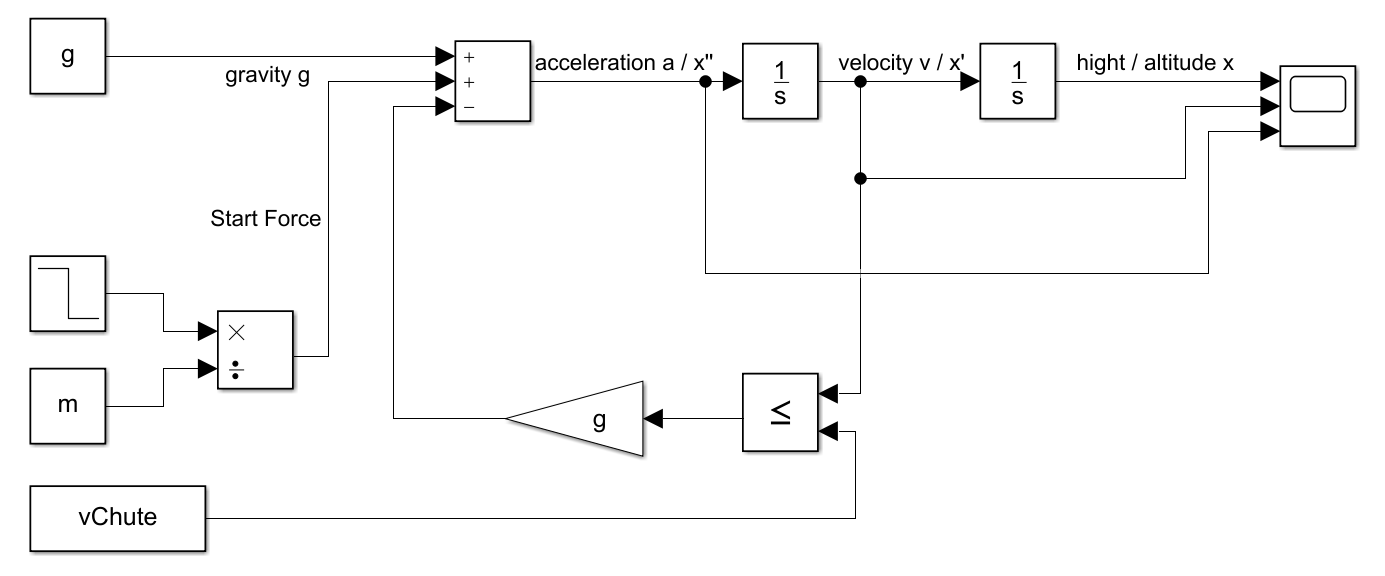
\includegraphics[width=0.7\textwidth]{figures/overview.png}
		\caption{Overview of the simulink model.}
		\label{fig:overview}
	\end{figure}


\section{Simulation}	
	
	\begin{figure}[H]
		\centering
		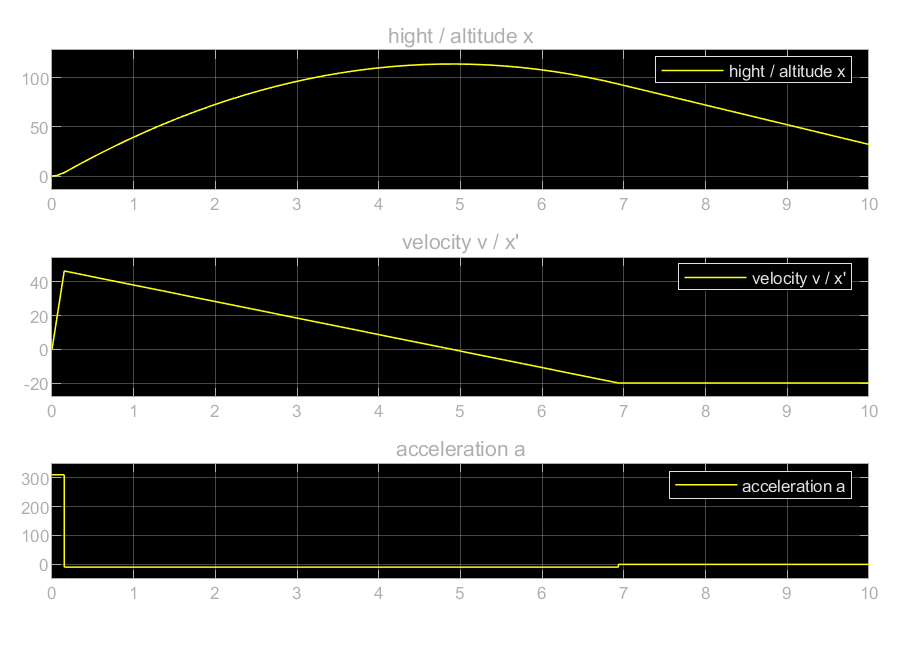
\includegraphics[width=0.7\textwidth]{figures/scope.eps}
		\caption{Scope from the Simulation.}
		\label{fig:scope1}
	\end{figure}
	
	
	
	

	\begin{lstlisting}
		clear all; clc; close all;
		
		%%
		% g inverted
		m=0.05; g=-9.81; tEngine=0.15; Force=16; vChute=-20; Dt=0.01; 
		clear t v h 
		n=1; 
		t(n)=0; v(n)=0; h(n)=0; t(2)=0;
		
		%%
		% Segment 1 
		a1=(Force-m*g)/m; 
		while (t(n) < tEngine) &&  (n < 50000) 
		n=n+1; 
		t(n)=t(n-1)+Dt; 
		v(n) =a1 *t (n) ; 
		h(n) =0.5*a1*t(n)^2;
		end;
		v1=v(n); h1=h(n); t1=t(n);
		
		% Segment 2
		while v(n)>=vChute && n<50000
		n=n+1;
		t(n)=t(n-1)+Dt;
		v(n)=v1-g*(t(n)-t1);
		h(n) =h1+v1 * (t(n)-t1 )-0.5*g* (t (n)-t1)^2;
		end
		v2=v(n); h2=h(n); t2=t(n);
		
		% Segment 3
		while h(n)>0 && n<50000
		n=n+1;
		t(n)=t(n-1)+Dt;
		v(n)=vChute;
		h (n) =h2+vChute* (t(n)-t2) ;
		end
		
		%%
		subplot(1,2,1)
		plot(t,h,t2,h2, 'ro', t1, h1, 'r+')
		xlabel('Time [s]');
		ylabel('Hight [m]');
		subplot(1,2,2)
		plot(t,v,t2,v2, 'ro', t1, v1, 'r+')
		xlabel('Time [s]');
		ylabel('Velocity [m]');
	\end{lstlisting}
	
%	\clearpage
%	\part{Theoretische Grundlagen}
%	\label{sec:theory}
%	\todo{Einführung schreiben}
%\clearpage
\section{Komponenten}

\todo{ evt. Skizze: Schon zu detailliert?}

Um die Zielsetzung zu erfüllen werden folgende Komponenten benötigt:

	\begin{description}
		\item[Wasserspeicher] \hfill \\ 
			Das Gerät kann selber einen Tank haben oder an die örtliche Wasserversorgung angeschlossen werden. Ein lokaler Tank müsste sicher ein Mehrfaches eines Trinkglases fassen. Sprich mehrere Liter.
		\item[Ventil] \hfill \\ 
			Damit soll der Wasserstrahl ein- und ausgeschaltet werden. Je nach bedarf muss er regulierbar sein.
		\item[Düse] \hfill \\
			Als Düse ist in der gesamten Dokumentation die Austrittsstelle des Wasser gemeint.
		\item[Sensorik] \hfill \\
			Es wird eine Sensorik benötigt um ein Glas zu erkennen und zu lokalisieren.
		\item[Mechanische Nachführung der Düse] \hfill \\
			Da das Wasser nicht ferngesteuert werden kann muss die Düse mechanisch seine Position verändern können. Es besteht jedoch auch die Möglichkeit, dass viele Düsen das Gebiet abdecken und jede ein separat angesteuertes Ventil hat.
		\item[Areal] \hfill \\
			Die Detektion und das füllen des Glases soll nur in einem begrenzten Gebiet realisiert werden.
			
	\end{description}
%\clearpage
\section{Sensorik}
%Auflösegenauigkeit
Um so genauer das Trinkglas detektiert werden kann, desto genauer kann die Düse schliesslich ausgerichtet werden. Daher ist eine präzise Lokalisierung des Trinkglases sehr wichtig. In einer ersten Abschätzung wird davon ausgegangen, dass eine Lokalisierung auf etwa $\pm$2cm genau ausreichend ist.\\
\todo{Abtastrate}
\todo{erkennen von Trinkglas? Nicht notwendig da Ventil manuell geöffnet wird?}

	\subsection{Bewertungskriterien}
		\begin{description}
			\item Abtastrate
			\item Kosten
			\item Aufwand
			\item Genauigkeit
			\item Platzbedarf
			\item Coolness
			\item Spezielles
			\item Lieferfristen
			
		\end{description}
	
	
	%\subsection{LIDAR}
	\subsection{Ultraschallsensor}
	%Ein Sensor oder mehrere
	Es wird ein Ultraschallsignal ausgesandt, dann wird die Zeit getoppt bis ein Echo wieder zurück beim Ausgangspunkt ist. Anhand dieser Zeit und der Schallgeschwindigkeit in der Luft wird die Distanz zwischen Sensor und dem Gegenstand berechnet.  \\
	Ultraschallsensoren haben meist eine grosse Detektionszone. Je nach Sensor und Distanz zum Teil bis zu 180°. Dies kann ein Vor- aber auch ein Nachteil sein. \todo{Vor und nachteile genauer ausformulieren}\\
	Mit drei Sensoren könnte man eine Position im Raum bestimmen. Da das Glas nicht genau definiert ist und so auch nicht der reflektierende Punkt verliert diese Methode stark an Genauigkeit. Es ist auch schwierig die Öffnung oben zu lokalisieren.
	
	\subsection{ToF - Time of Flight }% LiDAR}
	ToF ist die Abkürzung für Time of Flight und funktioniert ähnlich wie der Ultraschallsensor. Anstelle von Schallwellen wird Licht verwendet. Licht hat zwei markante Vorteil im Vergleich zum Schall. Einerseits ist es schneller, daher kann die Abtastrate erhöht werden. Andererseits, was wichtiger ist, kann Licht fokussiert werden. So kann nicht nur die Distanz sondern auch die Richtung und daraus die Position bestimmt werden.\\
	Da Glas lichtdurchlässig ist könnte es ein Problem sein, dass zu wenig Licht reflektiert wird und das Trinkglas so nicht detektiert wird. 
	
		\subsubsection{ToF-Kamera}
		Eine ToF-Kamera wäre wohl die einfachste Lösung. Sie liefert ein zweidimensionales Array mit Abstandswerten. Aufgrund der Daten könnte man mit herkömmlichen Bildverarbeitungsalgorithmen das Trinkglas vom Rest des Bildes extrahieren und so den Mittelpunkt der oberen Öffnung orten.\\		
		Die Frage welche sich hier stellt ist diejenige des Preises. 
		
		\subsubsection{Bewegbare Sensoren}
		Würde man einen oder mehrere Sensoren beweglich montieren könnte man das Areal abtasten und das Glas so detektieren.
		Diese Variante hat jedoch einige Nachteile. Es wird viel Zeit benötigt um das gesamte Areal abzutasten, es wird sehr schwierig den Bewegungen des Glases zu folgen und es ist kompliziert ein Trinkglas von einem anderen Gegenstand zu unterscheiden.
	
		\subsubsection{2D-Array aus Sensoren}
		Man könnte auch ein 2D-Array aus ToF-Sensoren machen und so das komplette Areal im Überblick halten. Wenn man für 40cm Breite alle 2cm einen Sensor nimmt, werden dafür schon 20 Sensoren gebraucht. Dies müsste man wohl noch mit Anzahl Sensoren in der Z-Achse multiplizieren.% und in der Höhe 
		
	
	\subsection{Lichtschranken}
	
	
	
	\subsection{Kamera}
	Wie das menschliche Gehirn die Bilder des Auges verarbeitet kann man Bilder von Digitalkameras verarbeiten. Dafür gibt es unterschiedliche Ansätze, aber im Prinzip würde man Farben und Formen erkennen um so das Trinkglas aus dem Hintergrund zu extrahieren.
	
		
		\subsection{2D-Kamera}
		\label{sec:2d}
		Eine einzelne Kamera füllt ein zweidimensionales Array mit Helligkeitswerten. 
		Daraus könnte man zum Beispiel den Boden oder die Öffnung extrahieren. Da ihre Durchmesser nicht exakt bekannt sind, ist es auch schwierig die genaue X- und Y-Position herauszulesen ausser das Glas ist Senkrecht über der Linse. \todo{Skizze}
		%Falls das Bild farbig ist enthält ein Punkt drei Farbwerte (je nach Farbsystem YCbCr, RGB, etc.)
		%So könnte man zum Beispiel den Kreisrunden Glasboden detektieren

		
		\subsection{3D-Kamera}
		Mit zwei etwas auseinander liegenden Kameras kann man ein Objekt dreidimensional erkennen. So kann auch der Mensch dank zwei Augen dreidimensional sehen. Man schaut wie weit der selbe Punkt auf den beiden Bildern auseinander liegt. Je weiter dieser auseinander liegt desto näher ist er. Sind die beiden Punkte am selben Ort so ist er in weiter Ferne. Dieses Verfahren heisst Stereovision.\\
		Es gäbe auch die Möglichkeit mit zwei Kameras aus verschiedenen Blickwinkeln das Areal zu beobachten.
		\todo{Skizze. Wird dieses Verfahren bereits irgendwo angewandt?}
		

		
		\subsection{Kamera und Distanzsensor}
		Würde man wie im Kapitel \ref{sec:2d} eine Kamera nehmen und zusätzlich noch einen Distanzsensor mit grossem Winkel, könnte man das Trinkglas im Raum genauer orten. Nur die Position der Öffnung lässt sich so nicht genau orten.
		
%\clearpage
\section{Nachführen des Wasserstrahls}

%Die Regelstrecke beinhaltet den mechanischen Teil zum Nachführen wie auch den Wasserstrahl. Einen kleinen Einfluss auf die Strecke dürfte auch das Ventil haben.
%\todo{Bild Übertragungsfunktion der Strecke/ Weg von Regelstrecke}


	\subsection{Bewertungskriterien der Nachführung}
		\begin{description}
			\item Totzeit des Wasserstrahls
			\item Kosten
			\item Aufwand
			\item Füllgeschwindigkeit
			\item Platzbedarf
			\item Coolness
			\item Spezielles 
			\item Lieferfristen
			
		\end{description}
	
	
	\subsection{Möglichkeit zum Nachführen der Düse}
		
		\subsubsection{Bogenstrahl}
		Diese Möglichkeit wurde in der Aufgabenstellung beschrieben. Die Düse hat einen festen Platz. Es wird lediglich ihr Winkel verändert um das Glas in einem Bogen zu treffen.
		
		\subsubsection{Nachführen auf der Ebene}
		Nach dem Vorbild eines 3D-Druckers soll bei dieser Variante die Düse in X- und Y-Achse bewegt werden. Bei Bedarf könnte man auch noch die Z-Achse mit einbeziehen.\\
		Anstelle von X und Y könnte man auch im Radialsystem arbeiten mit $\Phi$ und Radius.
		
		\subsubsection{Fläche mit Düsen}
		Anstelle die Düse zu Bewegen könnte man auch das komplette Areal mit Düsen abdecken. Hätte jede Düse ein eigenes Ventil käme man wohl auf über 100Ventile. Folgend eine Überschlagsrechnung mit einem Düsenabstand von 2cm. Eine Düse würde folglich $400m^2$ abdecken.
			\begin{equation}
				A = r^2 * \pi = \left( 200mm\right) ^2 * \pi = 62'832mm^2\\
				n = \frac{A_{Areal}}{A_{pro_Düse}} = \frac{62'832mm^2}{400mm^2} = 157
			\end{equation}
		Es gäbe noch die Variante, dass mehrere Ventile geöffnet werden müssen um bei einer Düse einen Wasserstrahl rauskommen zu lassen. Würden wir zum Beispiel die X- und Y- Achse einzeln ansteuern gäbe dies 30 Ventile bei gleichem Düsenabstand. \todo{Skizze}\\
		\todo{Optimieren der Anzahl....}
		
		\subsubsection{Drohne}
		Mit einer Flugdrohne hätte man wohl die grösste Flexibilität und könnte ohne grossen Aufwand ein viel grösseres Areal abdecken als vorgesehen. \\
		Würde man den Wassertank an der Drohne befestigen müsste diese vermutlich etwa 10kg Nutzlast fliegen können. Dies würde bedeuten, dass auch die Drohne dementsprechend viel Platz benötigt.\\
		Die andere Variante wäre die Drohne an eine "Leine" zu nehmen und das Wasser bei Bedarf über einen Schlauch hoch zu pumpen.
	
	
	\subsection{Bewertungen}
	
\section{Ventil}
\todo{Mögliche Ventile/ Wasserhähne raus suchen}
	
\section{Wassertank}



%\clearpage
\input{./tex/theory/conclusiontheory.tex}
%	\bookmarksetup{startatroot}
%	
%	\clearpage
%	\part{Simulationen}
%	\label{sec:simulation}
%	



\section{Regelkreis}

Das ganze System kann als geschlossener Reglerkreis dargestellt werden. Der Regler beinhaltet die ganze Sensorik und .....\\
Einheiten in Strecke\\
Störgrössen\\
Ist es eine Regelung oder eine Steuerung, da Sollwert geändert wird nicht aber der Standort rückgeführt wird?\\

	\subsection{Wasserstrahl}
	Abhängig von Distanz, Druck und Bogen wird der Wasserstrahl eine Totzeit haben. Auch ein gewisse Trägheit ist zu berücksichtigen.
	

%	
%	\clearpage
%	\part{Versuchsergebnisse}
%	\label{sec:experiment}
%	\input{experiment/experiment}
%	
%	\clearpage
%	\part{Schlussfolgerung}
%	\label{sec:conclusion}
%	

\section{Diskussion}

\section{Ausblick}


	
	%\clearpage
	%\part{Diskussion}
	%
	%\clearpage
	%\part{Ausblick}
	%	\label{sec:outlook}
	%	%\section{Ausblick}

\section{Untersuchungen}

%\subsection{Untersuchungen}
Mit den erzielten Resultaten ergeben sich weitere Fragestellungen,
welche in Folgearbeiten beantwortet werden sollten. Im Folgenden
soll zusammengefasst werden, welche Arbeiten und Untersuchungen
im Anschluss an die Arbeit durchzuführen sind.

\subsection{Alterungseinfluss auf die Modellparameter}
Die Arbeit stellt eine Möglichkeit vor, wie mit generischen
Modellparametern eine batteriespezifische Identifikation
umgangen werden kann. Der hierfür verwendete Stichprobenumfang,
auf welchem sich die getroffenen Annahmen stützen, ist mit
lediglich 10 Batterien sehr klein. Hierzu sind weitere
Batterien zu untersuchen, mit welchen für alle Batterietypen
belegt werden kann, dass der angenommene Alterungseinfluss
vorliegt.

\subsection{Einfluss des Ladens auf die SOC Schätzung}
Die Tests des realisierten Prototypen zeigen, dass die erzielten
\gls{soc} Schätzungen eine systematische Überschätzung während
der Erhaltungsladung zeigen. Die Validierung des 2-Puls Lasttest,
welche auch zur Ermittlung der Modellparameter diente, wurde ohne
gleichzeitiges Laden der Batterien durchgeführt. Um die
Modellparameter für den realen Einsatz mit gleichzeitiger
Ladung zu ermitteln, ist eine weitere Validierung unter diesen
Betriebsbedingungen durchzuführen. Alternativ ist eine Korrektur
der bereits angewendeten Modellparamer zu untersuchen, welche
empirisch aus den erzielten Testergebnissen zu bestimmen ist.

\subsection{Dauertest des Diagnosesystems}
Der realisierte Prototyp des Diagnosesystems ist gemäss dem
entwickelten Vorschlag fertigzustellen und einem Dauertest
zu unterziehen. Hierbei sollte insbesondere untersucht werden,
wie sich die Ergebnisse der \gls{soh} Schätzung entwickeln.
Zur Überprüfung sollte eine regelmässige Referenzmessung
durchgeführt werden, wie diese in der vorliegenden Arbeit
vorgestellt wurde.

\subsection{Modellparameter für weitere Temperaturen}
Die durchgeführte Validierung des 2-Puls Lasttest untersuchte
das Verfahren für zwei Temperaturen, für welche auch die
entsprechenden Modellparameter ermittelt wurden. Für die
Realisierung der vorgeschlagenen Temperaturkompensation,
welche den gesamten thermischen Einsatzbereich der
Batterien berücksichtigt, sind weitere Messungen notwendig.

\subsection{Kompensation der Batteriekabel}
Aufgrund der Tatsache, dass in der vorliegenden Anwendung
unterschiedliche Installationen mit verschiedenen Batteriekabeln
verwendet werden, wurde in der vorliegenden Arbeit eine direkte
Messung an den Batterieanschlüssen realisiert. Für die reale
Anwendung würde dies höhere Kosten der Verkabelung bedeuten.
Um diese zusätzlichen Kosten zu umgehen, könnte eine Korrektur
mittels einer Modellparametrierung eingesetzt werden. Hierzu
müssen die unterschiedlichen Verkabelungsvarianten untersucht
werden.

\section{Optimierungen}
Die vorliegende Arbeit zeigt auf, welche Faktoren den 2-Puls Lasttest
beeinflussen und  welche Performance mit dem realisierten \gls{bms}
erreicht werden kann. Die dabei festgestellten Verbesserungsmöglichkeiten
sollen im Folgenden zusammengefasst werden.

\subsection{Entladeregler}
Die Validierung des 2-Puls Lasttest zeigt, dass die Genauigkeit der
Schätzungen mit höheren Lastpulsen besser wird. Hierbei wird ein
Lastpuls von \SI{>2.4}{\ampere} empfohlen. Da mit der gegebenen
Hardware ausschliesslich Laspulse von $\leq \SI{1}{\ampere}$ realisiert
werden können, ist eine Modifikation für höhere Lastpulse in Betracht
zu ziehen.

\subsection{Temperaturmessung}
Die Untersuchung des bestehenden \gls{bms} zeigte, dass die
Temperaturmessung weder die Umgebungstemperatur noch die Temperatur
der Batterie misst. Diese misst die Temperatur der Leiterplatte,
auf welchem das \gls{bms} realisiert ist. Für den realisierten
Prototyp wurde deshalb auf eine Temperaturkompensation der
Modellparameter verzichtet. Um eine Temperaturkompensation
anzuwenden, bedarf es einer zuverlässigen Temperaturmessung.
Daher wird der Einsatz eines abgesetzten Temperatursensors
vorgeschlagen, welcher an der Batterie befestigt wird. Alternativ
ist auch der Einsatz einer Batterie mit integriertem
Temperatursensor denkbar.

\section{Einsatzstrategie}

Die vorliegende Arbeit befasst sich mit der Schätzung des
\gls{soh} und \gls{soc}. Die weitere Auswertung dieser
Werte wurde nicht behandelt. Für die Weiterentwicklung der
Anwendung wird empfohlen, diese Daten weiter auszuwerten.
Damit eine Weiterverarbeitung möglich ist, bedarf es einer
übergeordneten Strategie, welche definiert, was das
\gls{bms} diagnostizieren soll. Denkbar ist eine Beurteilung
der Einsatzfähigkeit für verschiedene Lastsituationen.
Damit könnte beurteilt werden, ob und wie lange gewissen
Lastsituationen durchführbar sind usw.


	%
	%% bibliography
	%\newpage
	%\cleardoublepage
	%\addcontentsline{toc}{section}{Literatur}
	%\bibliographystyle{ieeetr}
%\bibliographystyle{apalike}
%\bibliographystyle{alpha}

\bibliography{bib/bibliography.bib}
	%
	%
	%\addcontentsline{toc}{section}{Symbole}
	%\input{tex/symbols}
	%
	%% glossary
	%\newpage
	%\cleardoublepage
	%
	%%\clearpage
	%%\begin{multicols}{2}
	%%	\scriptsize
	%%	\glossarystyle{altlistgroup}
	%%	\glsaddall
	%	\printglossary[title=Glossar,nonumberlist]
	%	\printglossaries
	%%\end{multicols}
	%
	%% list of figures
	%\clearpage
	%%\newpage
	%%\cleardoublepage
	%% \phantomsection
	%\addcontentsline{toc}{section}{Abbildungen}
	%\listoffigures
	%
	%% lsit of tables
	%\clearpage
	%%\newpage
	%%\cleardoublepage
	%% \phantomsection
	%\addcontentsline{toc}{section}{Tabellen}
	%\listoftables
	%
%	 appendix
%	\clearpage
%	\begin{appendices}
%\pagenumbering{roman}

%\section{Aufgabenstellung}
%\includepdf[
%	pages=1-2,
%	offset=0 -2.2cm,
%	%frame,
%	width=0.8\textwidth,
%	picturecommand={\centering},
%	pagecommand={\thispagestyle{fancy}}
%	]{../../adm/aufgabenstellung/mission.pdf}

\iftoggle{printversion}{ % content for print version --------------------------
	\addtocontents{toc}{\protect\setcounter{tocdepth}{2}}
}{ % content for online version
	\addtocontents{toc}{\protect\setcounter{tocdepth}{3}}	
}

\end{appendices}

	
	
\end{document}
